\documentclass[a4paper,11pt]{scrartcl}
\usepackage{graphicx}
\usepackage[utf8]{inputenc}
\usepackage[T1]{fontenc}
\usepackage[ngerman]{babel}
\usepackage{bibgerm}
\usepackage{amsmath,amssymb,amsthm}
\usepackage{color}
\usepackage{enumerate}
\usepackage{tabularx}
\usepackage{subfig}
\usepackage{fancyhdr}
\usepackage{upgreek}
\usepackage{graphicx}
\usepackage{framed}
\usepackage{lmodern}
\usepackage{geometry}
\geometry{a4paper,left=20mm,right=30mm, top=3cm, bottom=2cm} 
\usepackage{marginnote}
\usepackage[pdftex,pdfpagelabels,colorlinks,backref,pagebackref,plainpages=false]{hyperref}
\setlength{\headwidth}{15cm}
\setlength{\textwidth}{15cm}

\usepackage{shadethm}
% == Set the heading style ===================================================
\setlength{\headheight}{14pt}
%\pagestyle{fancyplain}
\renewcommand{\sectionmark}[1]{\markboth{#1}{}}
\renewcommand{\subsectionmark}[1]{\markright{\thesection\ #1}}
\lhead[\fancyplain{}{\thepage}]{\fancyplain{}{\rightmark}}
\rhead[\fancyplain{}{\leftmark}]{\fancyplain{}{\thepage}}
\cfoot{}
\renewcommand{\headrulewidth}{0.4pt}
% ============================================================================

% == Set correct values for fitting floats ===================================
\tolerance=2000
\emergencystretch=10pt

\setcounter{topnumber}{3}
\setcounter{totalnumber}{5}
\setcounter{bottomnumber}{2}

% To make those darn floats fit where they should
\setcounter{totalnumber}{9}
\setcounter{topnumber}{9}
\setcounter{bottomnumber}{9}
\renewcommand{\textfraction}{0.00}
\renewcommand{\topfraction}{1.0}
\renewcommand{\bottomfraction}{1.0}
% ============================================================================

% == Abkürzungen für die reellen, natürlichen, ganzen,... Zahlen =============
\newcommand{\R}{{\ensuremath{\mathbb{R}}}}
\newcommand{\N}{{\ensuremath{\mathbb{N}}}}
\newcommand{\Z}{{\ensuremath{\mathbb{Z}}}}
\newcommand{\C}{{\ensuremath{\mathbb{C}}}}
\newcommand{\Q}{{\ensuremath{\mathbb{Q}}}}
\newcommand{\F}{{\ensuremath{\mathbb{F}}}}
\newcommand{\Prim}{{\ensuremath{\mathbb{P}}}}
% ============================================================================

\newcommand{\RM}[1]{\MakeUppercase{\romannumeral #1{}}} 

% == Makros für Autorenname und -adresse =====================================
\newcommand{\myaddress}[6]{%
  \parbox{\textwidth}{\textbf{\large #1}\\
    #2\\ #3\\ #4\\ 
    \ifthenelse{\equal{#5}{}}{}{Email: \href{mailto:#5}{\texttt{#5}}\\}
    \ifthenelse{\equal{#6}{}}{}{WWW: \href{#6}{\path|#6|}\\}
  } 
}

\newcommand{\myauthor}[1]{%
  \addtocontents{toc}{\protect\hspace{3.35ex}%
  \textsl{#1}\par}\vspace{-4ex}\quad\hfill\textsl{\Large #1}\vspace{8ex}}

\newcommand{\myname}[1]{\Large #1}

%%%%%%%%%%%%%%%%%%%%%%%%%%%%%%%%%%%%%%%%%%%%%%%%%%
% Tragen Sie in der folg. Zeile Ihren Namen ein: %
%%%%%%%%%%%%%%%%%%%%%%%%%%%%%%%%%%%%%%%%%%%%%%%%%%

\newcommand{\OO}{{\ensuremath{\mathcal{O}}}}
\newcommand{\const}{\ensuremath{\equiv}}

%\renewcommand{\thechapter}{\Roman{chapter}}
\renewcommand{\thesection}{\arabic{section}}


\newenvironment{Kasten}[1]
{
\hspace{0.05\linewidth}
\begin{center}
\begin{minipage}{0.95\linewidth}
\setlength{\fboxsep}{10pt}
%\setlength{\fboxsep}{18pt}
%\definecolor{shadecolor}{gray}{0.9}
\definecolor{shadecolor}{rgb}{0.9,1,1}
\definecolor{framecolor}{gray}{0}
%\def\FrameCommand{\fcolorbox{framecolor}{shadecolor}}
%\MakeFramed {\FrameRestore}
\subsubsection*{#1}
%\begin{itshape}
}
{
%\end{itshape}
%\endMakeFramed
\end{minipage}
\end{center}
%\vspace{1em}
}


\newenvironment{bsp}[1]
{
\setlength{\fboxsep}{10pt}
\subsection*{Beispiel: #1}
\begin{upshape}
}
{
\end{upshape}
}


\newenvironment{definition}[1]{
	\begin{definitions}
	\marginnote{\emph{#1}}
}{\end{definitions}}


\begin{document}
\pagenumbering{alph}
\begin{titlepage}
	\begin{center}	
		\LARGE \textbf{$n$-dimensionale Polarkoordinaten \\[5ex]
			{\Large Proseminar Mathematik - Themen zur Analysis \\[5ex] 
    		Wintersemester 2012/2013}\\[5ex]}
	\end{center}
	\begin{center}
		Simon Bischof; 06.12.2012
	\end{center}
\end{titlepage}
%\maketitle
\clearpage\pagenumbering{Roman}
\setcounter{tocdepth}{1}

\shorthandoff{"}
\clearpage\pagenumbering{arabic}
\section{Motivation}
Wenn mehrdimensionale Integrale in der Vorlesung eingeführt werden, d.h.
\begin{equation}
\label{int}
\int\limits_M f(x)dx \qquad (x\in\R^n,M\subseteq \R^n, f:\R^n\to\R),\end{equation}
ist eine der ersten Funktionen, die integriert wird, $f\const 1$. Damit wird der Inhalt (je nach Dimension Fläche, Volumen,$\ldots$) berechnet.\\
\includegraphics[scale=0.5]{images/nDWürfelKugel.jpg}\\
Für einfache Mengen wie den $n$-dimensionalen Würfel ist das mithilfe des Satzes von Fubini noch leicht machbar (man bekommt den Inhalt $1$). Für eine weitere regelmäßige Menge, die $n$-dimensionale Kugel $D(R)^n:=\{(x_1,\cdots,x_n)\in\R^n|x_1^2+\cdots+x_n^2\leq R^2\}$, ist das ganze ungleich komplizierter. Fubini liefert
$$\int\limits_{D(R)^n} d(x_1,\ldots,x_n)= \int\limits_0^R\int\limits_0^{\sqrt{R^2-x_1^2}}\int\limits_0^{\sqrt{R^2-x_1^2-x_2^2}}\ldots dx_3 dx_2 dx_1.$$
Nach Einführung der Polarkoordinaten lässt sich das Integral mithilfe der Substitutionsregel
\begin{equation}
\label{subst}
\int\limits_{g(A)}f(v)dv=\int\limits_A f(u)|\det(J_g(u))| du, \qquad g:A\to g(A) \text{injektiv.}
\end{equation}
viel einfacher berechnen.
\section{Grundlegendes}
\subsection{Vorgehensweise}
Die Polarkoordinaten werden als Funktion $P_n$ vom \glqq Polarkoordinatenraum\grqq{} in den kartesischen Raum induktiv definiert. Dabei dienen die bekannten Polarkoordinaten im Fall $n=2$ als Induktionsanfang. Außerdem werde ich immer noch den Fall $n=3$ explizit angeben, bei dem sich die ebenfalls bekannten Kugelkoordinaten ergeben.\\
Darauf werden einige Eigenschaften der Funktion $P_n$ bewiesen, insbesondere wird auch die Funktionaldeterminante berechnet, die für die Substitutionsregel \eqref{subst}
wichtig ist.\\
Bemerkung: $n$-dimensionale Polarkoordinaten lassen sich auch auf eine leicht andere Art und Weise definieren, so dass sie auch im Fall $n=1$ definiert sind. Außerdem ergeben sich dabei noch andere Vereinfachungen (Gleichbehandlung aller Winkelvariablen). Nachteil ist, dass sich dann für $n=2$ und $n=3$ nicht die bekannten Polar- bzw. Kugelkoordinaten ergeben.
\subsection{einige Definitionen}
\begin{itemize}
\item Es sei im Folgenden stets $n\in\N\setminus\{1\}$, denn für $n=1$ sind die Polarkoordinaten nicht definiert.
\item $e_n$ bezeichne den $n$-ten kanonischen Einheitsvektor. Soweit nichts anderes gesagt ist, sei $e_n\in\R^n$, also $e_n=(0,\ldots,0,1)^T$.
\item Als Skalarprodukt werde immer das Standardskalarprodukt im $\R^n$ verwendet, $||\bullet||$ sei im Folgenden die euklidische Norm.
\item Für Mengen $A\subset \R^n$ bezeichne $|A|$ das Volumen von $A$ gemäß \eqref{int} mit $f\const 1$.
\end{itemize}
\section{$P_n$: Definition und Eigenschaften}
\subsection{Definition}
$P_2:[0, \infty)\times [0, 2\pi]\to \R^2$ wird direkt definiert durch $P_2(r,\varphi_1)=\begin{pmatrix}
r\cos\varphi_1\\ r\sin\varphi_1\end{pmatrix}$.\\
Nun wird für $n>2$ die Funktion $P_n:[0,\infty)\times[0, 2\pi]\times[-\frac{\pi}{2},+\frac{\pi}{2}]^{n-2}\to \R^n$ induktiv definiert:\\[0.5em]
$P_n(r,\varphi_1, \varphi_2, \ldots, \varphi_{n-1})=\begin{pmatrix}
P_{n-1}(r,\varphi_1,\cdots,\varphi_{n-2})\cdot\cos\varphi_{n-1} \\ r\cdot\sin \varphi_{n-1}\end{pmatrix}
$ \\ $= \cos\varphi_{n-1}\begin{pmatrix}P_{n-1}(r,\varphi_1,\cdots,\varphi_{n-2}) \\ 0 \end{pmatrix}+r\sin\varphi_{n-1}e_n$\\
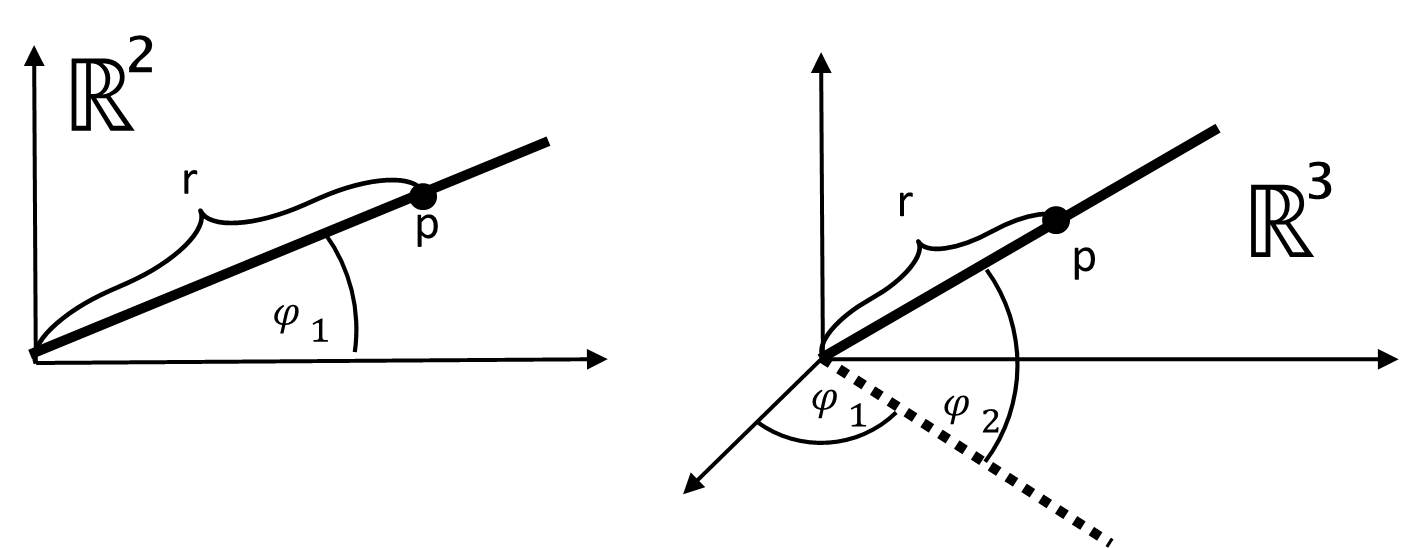
\includegraphics[scale=0.5]{images/PolarKugelkoordinaten.jpg}\\
Ausgeschrieben ergibt sich:\\
$P_n(r,\varphi_1, \varphi_2, \ldots, \varphi_{n-1})= \begin{pmatrix}r\cos\varphi_1\cos\varphi_2\cdot\ldots\cdot\cos\varphi_{n-1} \\ r\sin\varphi_1\cos\varphi_2\cdot\ldots\cdot\cos\varphi_{n-1} \\
r\sin\varphi_2\cos\varphi_3\cdot\ldots\cdot\cos\varphi_{n-1} \\
r\sin\varphi_3\cos\varphi_4\cdot\ldots\cdot\cos\varphi_{n-1} \\
\vdots \\
r\sin\varphi_{n-2}\cos\varphi_{n-1} \\
r \sin\varphi_{n-1}
\end{pmatrix}$\\
Im Falle $n=3$ ergeben sich daher die bekannten Kugelkoordinaten
$$P_3(r,\varphi_1, \varphi_2)=
\begin{pmatrix}r\cos\varphi_1\cos\varphi_2 \\
r\sin\varphi_1\cos\varphi_2\\
r\sin\varphi_2\\ \end{pmatrix}$$

\subsection{$||P_n(r,\varphi_1,\cdots,\varphi_{n-1})||$}
Im Falle $n=2$ ergibt sich durch direktes Ausrechnen:\\
$||P_2(r,\varphi_1)||^2=||\begin{pmatrix}r\cos\varphi_1\\ r\sin\varphi_1\end{pmatrix}||^2=
r^2\cos^2\varphi_1+r^2\sin^2\varphi_1=r^2\cdot(\cos^2\varphi_1+\sin^2\varphi_1)=r^2$.\\
Wegen $r\geq 0$ gilt also $||P_2(r,\varphi_1)||=r$.\\
Ebenso ist ($n=3$): $||P_3(r,\varphi_1,\varphi_2)||^2=
||\begin{pmatrix}r\cos\varphi_1\cos\varphi_2\\ r\sin\varphi_1\cos\varphi_2\\ r\sin\varphi_2\end{pmatrix}||^2=
r^2\cos^2\varphi_1\cos^2\varphi_2+r^2\sin^2\varphi_1\cos^2\varphi_2+r^2\sin^2\varphi_2
=r^2\cos^2\varphi_2+r^2\sin^2\varphi_2=r^2$, also wieder $||P_3(r,\varphi_1,\varphi_2)||=r$.\\ \\
Der Beweis, dass tatsächlich $||P_n(r,\varphi_1,\ldots,\varphi_{n-1})||=r$ für alle $n$ gilt, erfolgt mit vollständiger Induktion:\\
\textbf{Induktionsanfang:} Für $n=2$ wurde dies oben schon gezeigt. \checkmark\\
\textbf{Induktionsvoraussetzung:} Es sei $||P_n(r,\varphi_1,\ldots,\varphi_{n-1})||=r$.\\
\textbf{Induktionsschritt:} Es ist leicht einzusehen, dass $(P_n(r,\varphi_1, \varphi_2, \ldots, \varphi_{n-1}), 0)\cdot e_{n+1} = 0$. 
Also gilt mit dem Satz des Pythagoras:\\
$||P_{n+1}(r,\varphi_1,\ldots,\varphi_n)||^2=\cos^2\varphi_n\cdot||P_n(r,\varphi_1,\ldots,\varphi_{n-1})||^2 +\sin^2\varphi_n\cdot||r\cdot e_{n+1}||^2=r^2\cos^2\varphi_n+r^2\sin^2\varphi_n=r^2$ \checkmark

\subsection{Funktionalmatrix und -determinante}
Zuerst untersuchen wir die 2- und 3-dimensionalen Polarkoordinaten. Für $P_2$ ist, wie direkt nachzurechnen,\\
$J_{P_2}(r,\varphi_1)=\begin{pmatrix}\cos\varphi_1 & -r\sin\varphi_1 \\
\sin\varphi_1 & r\cos\varphi_1\end{pmatrix}$. Die Fuktionaldeterminante ist 
$$\det (J_{P_2}(r,\varphi_1))=\det\begin{pmatrix}\cos\varphi_1 & -r\sin\varphi_1 \\
\sin\varphi_1 & r\cos\varphi_1\end{pmatrix}=r\cos^2\varphi_1+r\sin^2\varphi_1 =r(\cos^2\varphi_1+\sin^2\varphi_1)=r.$$
Im Fall $n=3$ ist \\
$J_{P_3}(r, \varphi_1, \varphi_2 )=
\begin{pmatrix} \cos\varphi_1\cos\varphi_2 & -r\sin\varphi_1\cos\varphi_2 & -r\cos\varphi_1\sin\varphi_2 \\ 
\sin\varphi_1\cos\varphi_2 & r\cos\varphi_1\cos\varphi_2 & -r\sin\varphi_1\sin\varphi_2 \\
\sin\varphi_2 & 0 & r\cos\varphi_2 \end{pmatrix}$ und mit Sarrus\\
$\det(J_{P_3}(r, \varphi_1, \varphi_2 ))=
\det\begin{pmatrix} \cos\varphi_1\cos\varphi_2 & -r\sin\varphi_1\cos\varphi_2 & -r\cos\varphi_1\sin\varphi_2 \\ 
\sin\varphi_1\cos\varphi_2 & r\cos\varphi_1\cos\varphi_2 & -r\sin\varphi_1\sin\varphi_2 \\
\sin\varphi_2 & 0 & r\cos\varphi_2 \end{pmatrix}\\
=r^2\cos^2\varphi_1\cos^3\varphi_2+ r^2\sin^2\varphi_1\sin^2\varphi_2\cos\varphi_2+ r^2\sin^2\varphi_1\cos^3\varphi_2 + r^2\cos^2\varphi_1\sin^2\varphi_2\cos\varphi_2 \\
= r^2\cos\varphi_2(\cos^2\varphi_1\cos^2\varphi_2+\sin^2\varphi_1\sin^2\varphi_2+\sin^2\varphi_1\cos^2\varphi_2 + \cos^2\varphi_1\sin^2\varphi_2) \\
=r^2\cos\varphi_2(\cos^2\varphi_1(\cos^2\varphi_2+\sin^2\varphi_2)+ \sin^2\varphi_1(\cos^2\varphi_2+\sin^2\varphi_2))\\ =r^2\cos\varphi_2(\cos^2\varphi_1+\sin^2\varphi_1)=r^2\cos\varphi_2.$\\
Wir berechnen nun für allgemeines $n$ die Spalten der Funktionalmatrix separat.\\
Zur Vereinfachung der Rechnung setzen wir $\bar{P}_n(r,\varphi_1,\ldots,\varphi_{n-1})=\begin{pmatrix}P_n(r,\varphi_1,\ldots,\varphi_{n-1}) \\ 0 \end{pmatrix}\cdot\cos\varphi_n$.\\
Da $\cos\varphi_n$ und $\sin\varphi_n$ nicht von $r$ oder $\varphi_k \quad (k=1,\ldots,n-1)$ abhängen und $P_n(r,\varphi_1,\ldots,\varphi_{n-1})$ nicht von $\varphi_n$, gilt:\\[1.5em]
$ \partial_r P_{n+1}(r,\varphi_1,\ldots,\varphi_n)= \partial_r (\bar{P}_n(r,\varphi_1,\ldots,\varphi_{n-1})\cdot\cos\varphi_n) + \partial_r (r\sin\varphi_n e_{n+1})= \partial_r \bar{P}_n(r,\varphi_1,\ldots,\varphi_{n-1})\cdot\cos\varphi_n + \sin\varphi_n e_{n+1} = \begin{pmatrix}\partial_r P_n(r,\varphi_1,\ldots,\varphi_{n-1})\cdot\cos\varphi_n \\ \sin\varphi_n \end{pmatrix} $\\[1.5em]
$ \partial_{\varphi_k}P_{n+1}(r,\varphi_1,\ldots,\varphi_n) = \partial_{\varphi_k} (\bar{P}_n(r,\varphi_1,\ldots,\varphi_{n-1})\cdot\cos\varphi_n) + \partial_{\varphi_k} (r\sin\varphi_n e_{n+1})= \partial_{\varphi_k} \bar{P}_n(r,\varphi_1,\ldots,\varphi_{n-1})\cdot\cos\varphi_n = \begin{pmatrix}\partial_{\varphi_k} P_n(r,\varphi_1,\ldots,\varphi_{n-1})\cdot\cos\varphi_n \\ 0 \end{pmatrix} \qquad (k=1,\ldots,n-1)$\\[1.5em]
$ \partial_{\varphi_n}P_{n+1}(r,\varphi_1,\ldots,\varphi_n)=\partial_{\varphi_n}(\bar{P}_n(r,\varphi_1,\ldots,\varphi_{n-1})\cdot\cos\varphi_n) + \partial_{\varphi_n} (r\sin\varphi_n e_{n+1})=-(\bar{P}_n(r,\varphi_1,\ldots,\varphi_{n-1})\cdot\sin\varphi_n+r\cos\varphi_n e_{n+1} = \begin{pmatrix}-P_n(r,\varphi_1,\ldots,\varphi_{n-1})\cdot\sin\varphi_n \\ r\cos\varphi_n \end{pmatrix} $\\[1.5em]
Behauptung:
\begin{equation}
\label{det}\det(J_{P_{n+1}}(r,\varphi_1,\ldots,\varphi_n))=\det(J_{P_n}(r,\varphi_1,\ldots,\varphi_{n-1}))\cdot r\cos^{n-1}\varphi_n
\end{equation}
Für $\cos\varphi_n=0$ ist wegen $\partial_{\varphi_1}P_{n+1}(r,\varphi_1,\ldots,\varphi_n)=0$ schon $\det(J_{P_{n+1}}(r,\varphi_1,\ldots,\varphi_n))=0$.\\
Für $\cos\varphi_n\neq 0$ schließlich addiert man das $r\sin\varphi_n(\cos\varphi_n)^{-1}$-fache der ersten zur letzten Spalte. Da $r\partial_r P_n(r,\varphi_1,\ldots,\varphi_{n-1})=P_n(r,\varphi_1,\ldots,\varphi_{n-1})$, geht diese in $r(\cos\varphi_n)^{-1}e_n$ über. Wenn man nach der letzten Spalte dann entwickelt, entsteht in der Restmatrix gerade $\cos\varphi_n J_{P_n}(r,\varphi_1,\ldots,\varphi_{n-1})$.\\
Also ist $\det(J_{P_{n+1}}(r,\varphi_1,\ldots,\varphi_n))=r(\cos\varphi_n)^{-1}\det(\cos\varphi_n J_{P_n}(r,\varphi_1,\ldots,\varphi_{n-1})) = r(\cos\varphi_n)^{n-1}\det(J_{P_n}(r,\varphi_1,\ldots,\varphi_{n-1}))$. Daher gilt \eqref{det}.
Damit und mit $\det(J_{P_2}(r, \varphi_1))=r$ folgt rekursiv:\\
Es gilt $\det(J_{P_n}(r,\varphi_1,\ldots,\varphi_{n-1}))=|\det(J_{P_n}(r,\varphi_1,\ldots,\varphi_{n-1}))|=r^{n-1}\prod\limits_{i=2}^{n-1}\cos^{i-1}\varphi_i$.
\section{Integralberechnungen}
\subsection{Die Gammafunktion $\Gamma$}
Um das Volumen der Kugel auszurechnen, benötigt man die Gammafunktion \\$\Gamma:\underbrace{\R\setminus(-\N_0)}_{:=B}\to\R$ (sie ist auf ganz $\C\setminus(-\N_0)$ erklärt, was wir hier aber nicht brauchen). Einige wichtige Eigenschaften werden hier ohne Beweis angegeben:
\begin{itemize}
\item $\Gamma(x+1)=x\cdot\Gamma(x) \quad (x\in B)$
\item $\Gamma(1)=1\Rightarrow\Gamma(k)=(k-1)!\quad (k\in\N)$
\item $\Gamma(\frac{1}{2})=\sqrt{\pi}\Rightarrow\Gamma(n+\frac{1}{2})=\sqrt{\pi}\cdot\frac{1}{2}\cdot\frac{3}{2}\cdot\ldots\cdot (n-\frac{1}{2})=\left(\frac{1}{2}\right)^n\sqrt{\pi}\cdot 1\cdot 3\cdot\ldots\cdot (2n-1)\quad (n\in\N)$
\item und $\int\limits_0^1 (1-t)^{w-1}\cdot t^{z-1}dt=\frac{\Gamma(z)\Gamma(w)}{\Gamma(z+w)} \quad (z,w\in B)$\\ (siehe z.B. Königsberger, Analysis 2, Kapitel 6.6)
\end{itemize}
\subsection{Inhalt der $n$-dimensionalen Kugel}
Sei $\kappa_n:=|D(R)^n|$, mit $R>0$ fest. Sei $A:=[0,R]\times[0,2\pi]\times[-\frac{\pi}{2},+\frac{\pi}{2}]^{n-2}$. Dann ist $P_n(A)=D(R)^n$. Nun ist aber $P_n$ auf $A$ nicht injektiv.\\
Allerdings ist $\{x\in A|\exists y\in A: x\neq y \wedge P_n(x)=P_n(y)\}$ eine Lebesgue-Nullmenge. Also darf man die Substitutionsregel \eqref{subst} anwenden. Sie liefert
\[\int\limits_{D(R)^n}dx=\int\limits_A |\det(J_{P_n}(r,\varphi_1,\ldots,\varphi_{n-1}))|d(r,\varphi_1,\ldots,\varphi_{n-1})=
\int\limits_A r^{n-1}\prod\limits_{i=2}^{n-1}\cos^{n-1}\varphi_i d(r,\varphi_1,\ldots,\varphi_{n-1}) \]
\begin{equation}\label{kappa}\stackrel{Fubini}{=}\int\limits_0^R r^{n-1}dr\cdot\int\limits_0^{2\pi}d\varphi_1\cdot \\ \prod\limits_{i=2}^{n-1}\left(\int\limits_{-\frac{\pi}{2}}^\frac{\pi}{2} \cos^{i-1}\varphi_i d\varphi_i\right)
\end{equation}
Wir berechnen die Faktoren von \eqref{kappa} einzeln:
Zuerst ist $\int\limits_0^{2\pi}d\varphi_1=2\pi$ und $\int\limits_0^R r^{n-1}dr=\left[\frac{r^n}{n}\right]_0^R=\frac{R^n}{n}$. Außerdem:
$$\int\limits_{-\frac{\pi}{2}}^\frac{\pi}{2} \cos^{n-1}\varphi_n d\varphi_n=\int\limits_{-\frac{\pi}{2}}^\frac{\pi}{2} \sqrt{1-\sin^2\varphi_n}^{n-1} d\varphi_n$$
$$\left. \begin{array}{c} \varphi_n= \arcsin \xi \\ d\varphi_n = \frac{1}{\sqrt{1-\xi^2}}d\xi\end{array}\right|
=\int\limits_{-1}^1 \sqrt{1-\xi^2}^{n-2}d\xi=2\int\limits_0^1\sqrt{1-\xi^2}^{n-2}d\xi$$
$$\left. \begin{array}{c} \xi= \sqrt{t} \\ d\xi = \frac{1}{2\sqrt{t}}dt\end{array}\right|
=\int\limits_0^1 (1-t)^\frac{n-2}{2}t^{-\frac{1}{2}}dt = \int\limits_0^1 (1-t)^{\frac{n}{2}-1}t^{\frac{1}{2}-1}dt
=\frac{\Gamma(\frac{1}{2})\Gamma(\frac{n}{2})}{\Gamma(\frac{n+1}{2})}$$
Im zweidimensionalen ist damit $\kappa_2=\int\limits_0^R rdr\cdot \int\limits_0^{2\pi}d\varphi_1 d\varphi_1=\frac{R^2}{2}\cdot 2\pi=\pi R^2$.\\
In $\R^3$ ist $\kappa_3=\int\limits_0^R rdr\cdot \int\limits_0^{2\pi}d\varphi_1 d\varphi_1\cdot \int\limits_{-\frac{\pi}{2}}^\frac{\pi}{2} \cos\varphi_2 d\varphi_2=\frac{R^3}{3}\cdot 2\pi\cdot[\sin\varphi_2]_{-\frac{\pi}{2}}^\frac{\pi}{2}=\frac{4\pi}{3} R^3$.\\
Nun zum allgemeinen Teil:\\
$\kappa_n=2\pi\frac{R^n}{n}\prod\limits_{k=2}^{n-1}\left(\int\limits_{-\frac{\pi}{2}}^\frac{\pi}{2}\cos^{k-1}\varphi_k d\varphi_k\right)=2\pi\frac{R^n}{n}\cdot\sqrt{\pi}^{n-2}\cdot\frac{\Gamma(1)}{\Gamma(\frac{3}{2})}\cdot\frac{\Gamma(\frac{3}{2})}{\Gamma(2)}\cdot\ldots\cdot\frac{\Gamma(\frac{n-1}{2})}{\Gamma(\frac{n}{2})}
\\=\begin{cases}\frac{2\sqrt{\pi}^n R^n}{(q-1)!\cdot n}; \qquad n=2q, q\in\N \\ \frac{2^{q+1}\sqrt{\pi}^{n-1}R^n}{1\cdot 3\cdot 5\cdot \ldots\cdot(n-2)\cdot n}; \qquad n=2q+1, q\in\N\end{cases}$\\
$=\begin{cases}\frac{\pi^q R^{2q}}{q!}; \qquad n=2q, q\in\N \\ \frac{2^{q+1}\sqrt{\pi}^q R^{2q+1}}{1\cdot 3\cdot \ldots\cdot (2q+1)} \qquad n=2q+1, q\in\N\end{cases} $
\subsection{Sonstiges}
Nun können wir auch andere Funktionen integrieren. Beispielsweise sei $f(x)=x_n\sqrt{x_1^2+\ldots x_n^2}$. Dann ist $\int\limits_{D(R)^n}f(x)dx=\int\limits_A r^2\sin\varphi_{n-1}r^{n-1}\prod\limits_{i=2}^{n-1}\cos^{n-1}\varphi_i d(r,\varphi_1,\ldots,\varphi_{n-1})$. Dies lässt sich dann wie vorher ausrechnen.
\section{Verallgemeinerungen}
Selsbstverständlich lassen sich auch viele Variationen und Verallgemeinerungen zu den Polarkoordinaten finden. Zwei hilfreiche Verallgemeinerungen werden hier kurz angedeutet.
\subsection{\glqq Ellipsoidkoordinaten\grqq}
Seien $a_1,\ldots,a_n>0$ fest. Die Menge $M^n:=\{x\in\R^n|\frac{x_1^2}{a_1^2}+\ldots\frac{x_n^2}{a_n^2}=1\}$ ist ein $n$-dimensionales Ellipsoid mit den Halbachsen $a_1,\ldots,a_n$. Im Spezialfall $a_1=\ldots=a_n:=r$ wird $M^n$ zu einer $n$-dimensionalen Kugel mit Radius $r$.\\
Mithilfe einer modifizierten Form von $P_n$, nämlich\\ $Q_n(r,\varphi_1,\ldots,\varphi_{n-1})=\begin{pmatrix}a_1r\cos\varphi_1\cdot\ldots\cdot\cos\varphi_{n-1} \\ a_2r\sin\varphi_1\cdot\ldots\cdot\cos\varphi_{n-1} \\
a_3r\sin\varphi_2\cdot\ldots\cdot\cos\varphi_{n-1} \\
\vdots \\
a_nr \sin\varphi_{n-1}
\end{pmatrix}=\begin{pmatrix}a_1 & & & \\ & a_2 & & \\ & & \ddots & \\ & & & a_n\end{pmatrix}\cdot P_n(r,\varphi_1,\ldots,\varphi_{n-1})$,
lässt sich der Inhalt von $M^n$ leicht berechnen. Es ist dann für $A:=[0,1]\times[0,2\pi]\times[-\frac{\pi}{2},+\frac{\pi}{2}]^{n-2}$: $Q_n(A)=M^n$. Wegen $\det(BC)=\det(B)\det(C)$ gilt:\\
$|\det(J_{Q_n}(r,\varphi_1,\ldots,\varphi_{n-1}))|=
a_1\cdot a_2\cdot\ldots\cdot a_n\cdot|\det(J_{P_n}(r,\varphi_1,\ldots,\varphi_{n-1}))|$.\\
Damit ist auch $|M^n|=\int\limits_{M^n}dx=\int\limits_A |\det(J_{Q_n}(r,\varphi_1,\ldots,\varphi_{n-1}))|d(r,\varphi_1,\ldots,\varphi_{n-1})=a_1 a_2 \ldots a_n \int\limits_A |\det(J_{P_n}(r,\varphi_1,\ldots,\varphi_{n-1}))|d(r,\varphi_1,\ldots,\varphi_{n-1})=a_1 a_2 \ldots a_n |D(1)^n|$.
\subsection{verallgemeinerte Zylinderkoordinaten}
Man kann die Polarkoordinaten und die kartesischen Koordinaten kombinieren. Das bekannteste Beispiel sind die Zylinderkoordinaten im $\R^3$, deren erste zwei Komponenten 2-dimensionale Polarkoordinaten sind und deren dritte Komponente eine kartesische Koordinate ist. Die $(n+k)$-dimensionalen Zylinderkoordinaten verallgemeinern diese. Dabei stehe $n$ wie bisher für die Dimension der Polarkoordinaten und $k$ für die Dimension der Zylinderkoordinaten. Für $k=0$ ergeben sich die $n$-dimensionalen Polarkoordinaten.\\
Wir definieren $Q_{n,k}:[0,\infty)\times[0, 2\pi]\times[-\frac{\pi}{2},+\frac{\pi}{2}]^{n-2}\times \R^k\to\R^{n+k}$ durch
$$Q_{n,k}(r,\varphi_1,\ldots,\varphi_{n-1}, x_1, \ldots, x_k)=
\begin{pmatrix} \\ P_n(r,\varphi_1,\ldots,\varphi_{n-1}) \\ \\ 0 \\ \vdots \\ 0 \end{pmatrix}
+ \begin{pmatrix} 0 \\ \vdots \\ 0 \\ x_1 \\ \vdots \\ x_k \end{pmatrix}.$$
Für die Jacobimatrix gilt $$J_{Q_{n,k}}(r,\varphi_1,\ldots,\varphi_{n-1}, x_1, \ldots, x_k)=\begin{pmatrix}
J_{P_n}(r,\varphi_1,\ldots,\varphi_{n-1}) & 0 \\ 0 & I_k
\end{pmatrix}$$
(wobei $I_k\in\R^{k\times k}$ Einheitsmatrix). Aufgrund der Blockform ist \\$\det (J_{Q_{n,k}}(r,\varphi_1,\ldots,\varphi_{n-1}, x_1, \ldots, x_k)) = \det (J_{P_n}(r,\varphi_1,\ldots,\varphi_{n-1}))\cdot \det I_k=\det (J_{P_n}(r,\varphi_1,\ldots,\varphi_{n-1}))$.\\
Seien $R,l_1,l_2,\ldots,l_k>0$, $A:=D(R)^n\times[0,l_1]\times[0,l_2]\times\ldots\times[0,l_k]$ und $B:=[0,\infty)\times[0, 2\pi]\times[-\frac{\pi}{2},+\frac{\pi}{2}]^{n-2}\times[0,l_1]\times[0,l_2]\times\ldots\times[0,l_k]$. Dann ist $Q_{n,k}(B)=A$ und somit
$$|A|=\int\limits_A d(r,\varphi_1,\ldots,\varphi_{n-1}, x_1, \ldots, x_k)$$
$$=\int\limits_B |\det (J_{Q_{n,k}}(r,\varphi_1,\ldots,\varphi_{n-1}, x_1, \ldots, x_k))| d(r,\varphi_1,\ldots,\varphi_{n-1}, x_1, \ldots, x_k)$$
$$ = \int\limits_B |\det (J_{P_n}(r,\varphi_1,\ldots,\varphi_{n-1}))| d(r,\varphi_1,\ldots,\varphi_{n-1}, x_1, \ldots, x_k) = l_1 l_2 \ldots l_k \cdot |D(R)^n|.$$
\section{Quellen}
\begin{itemize}
\item Königsberger, Analysis 2 (S. 18f, 91f, 225-227, 287f)
\item HM-Vorlesung von Herrn Dr. Herzog (WS 2010/11, SS 2011)
\end{itemize}
\end{document}